\section{Experimental Results}
\label{sec:eval}

In this section we present our experimental results 
to show the accuracy and efficiency 
of our atomatic list items extraction algorithm. 
We first discuss the experimental setup,
including system overview, benchmark generation,
and experimental environment.
Then we present the longitudinal comparison between different version of our system,
which shows the performance improvement of our optimization.
Thirdly, we present a horizontal comparison 
between our system and MDR \cite{LiuGZ03:MDR} system,
which shows advandtage of our system in both accuracy and efficiency. 
Finally, we discuss about the title extraction.
Each of the latter three subsection contains three parts:
Evaluation Metrics,
Accuracy Analysis,
and Efficiency Analysis.

\subsection{Experimental Setup}
\subsubsection{System Overview}
Our System contains two mode:
Single Page Mode and Benchmark Test Mode.
In Single Page Mode,
given the URL of a web page and the number of desired list items, 
our system can extract the data record list and save the result in a text file. 
Figure \ref{fig:snapshotOfSystem}(a) shows the extraction result 
of the given web page 
which is presented by figure \ref{fig:snapshotOfWebPage}. 

In Benchmark Test Mode,
the system will read the benchmark file and load the cached pages 
from designated address,
The system will extract the lists of all the benchmark pages and save the result in a text file. 
Figure \ref{fig:snapshotOfSystem}(b) shows the extraction result 
of the benchmark test.

The system also offer a option to enable the title extraction.
The system will extract the data record titles of the pages if we enable this function.
Otherwise, the system will extract the plain text of each data records.


\subsubsection{Benchmark Generation}
In order to evaluate our extraction system automatically, we first design benchmark. Test cases in benchmark are collected from the whole Internet. Our goal is to extract list items from the whole Internet not to extract list items from particular websites.

In collection phrase, we use a paradigm-superlative Number Object- which indicates the web page contains a list of N items in the same topic. We first google an instance of the paradigm such as Best 10 Players, then we collect the search result using a heuristics. By using different instances of the paradigm, we collect 100 web pages from different websites and domains.

After collection, we label the cached web pages. 
For each web page, 
we label the first item of data record list which we want to extract.

Finally we generate two benchmarks B1 and B2
which have 92 pages and 96 pages respectively.
And there are no overlapping between them.

In order to compare with MDR\cite{LiuGZ03:MDR} system,
we generate another benchmark B3 
from the testbed\cite{deepwebtestbed} 
which is used in Gengxin Miao's paper\cite{MiaoTHSM09:TagPathClustering}.
The testbed is designed for information extraction from the deep Web,
which has 253 Web pages from 51 web sites randomly 
drawn from 114,540 web pages with search forms.
We randomly choose 142 pages from 29 web sites to form B3.
Since our system needs to know the list item number $k$ of the page,
we manually assign the list number $k$ for each page in the benchmark.
Also we label the first item of data record list of each page.

\subsubsection{Experimental Environment}
Our experiments were carried out on a Core(TM)2 computer
with a 2GHz Due CPU and 3G of RAM. Our C\# im-
plementation of the algorithm utilizes the open source 
HTML parser Winista HtmlParser{\bf ref}. 
Also we use GoogleSearchAPI.Net20 to generate our benchmark B1 and B2

\subsection{Horizontal Comparison}

\subsubsection{Evaluation Metrics}
%Since all the test cases of benchmarks contain a correct data record list 
%that we want to extract.

Given a page $p$ for evaluation, 
we have the extracted list items $S_l$. 
If one of the items in $S_l$ contains our mannually added label, 
then we consider this page are extracted correctly.

Here we use precision and recall as the evaluation metrics for our system's accuracy test. 
The precision($P$) and recall($R$) are defined straightforwardly as follows:

\begin{equation}
	P = \frac{|correctly\,extracted\,pages|}{|pages\,with\,returned\,list\,items|}
\end{equation}

\begin{equation}
	R = \frac{|correctly\,extracted\,pages|}{|number\,of\,testcases\,in\,benchmark|}
\end{equation}

\subsubsection{Evaluation Result}
We keep two versions of our system:
the original version V1
and the lastest version V2.
V1 implements the basic algorithm 
while V2 contains the three optimization mentioned in approach section.
The result of our experiment is shown in Figure ?? and 
the average accuracy is shown in \ref{tab:EvalRes1}.

\begin{table}[tb]
\centering
\caption{Average Accuracy comparison}
\label{tab:EvalRes1}
\begin{tabular}{|c||c|c|} 
\hline
Version & P & R\\\hline
V1 (\%)& 87.3 & 59.5 \\\hline
V2 (\%)& 90.3 & 70.9 \\\hline
\end{tabular}
\end{table}
{\bf the results of V1 needs to be test again,and one more figure}

From the result we can see several points
First, the original version can basically solve our problem with an acceptable outcome.
Second, our optimizations can effectively improve the performance,
thus our final version can offer a relatively high recall and precision score.
The result of B3 is higher than the previous two benchmarks
since the deep web pages are more neat in HTML structures.

%Using two totally different benchmarks, the accuracy performance of our extraction algorithm is shown by figure \ref{fig:PR}. 
%The high precision indicates that our approach is effective to extract list items from syntactically repetitive web pages. 
%As for the benchmark is collected from the whole Internet, 
%the moderate recall indicates that our approach is suitable for web scale extraction.

%\begin{figure}
%	\includegraphics[width=8cm]{./PR.eps}
%	\caption{Precision and Recall}
%	\label{fig:PR}
%\end{figure}

\subsubsection{Efficiency Test}
We design two experiments to test our approach's efficiency. In table \ref{tab:TimeCostDistribution}, we discuss the time cost of our approach. For one-hundred web pages, the extrextion module only costs 1.1835s. Figure \ref{fig:FileSize} and figure \ref{fig:ListSize} conclude another experiment. Figure \ref{fig:FileSize} shows that the time cost of extraction algorithm is in direct proportion to web page size and figure \ref{fig:ListSize} shows that list size doesn't affect extraction time.

\begin{table}[tb]
\centering
\caption{Execution Time of Different Stages}
\label{tab:TimeCostDistribution}
\begin{tabular}{|c|c||c|c|c|c|c|c|c|c|} 
\hline
Version & Item & Total & I/O & Parsing & Tag Path Gen. & Labeling & Growing up & Interleaving & Other\\\hline
V1 & Time(ms) &  & 11.80 & 7.49 & 1.18 & 2.75\\\hline
V1 & Pct (\%) & $<1$ & 51 & 32 & 5 & 12\\\hline
V2 & Time(s) & 0.12 & 11.80 & 7.49 & 1.18 & 2.75\\\hline
V2 & Pct (\%) & $<1$ & 51 & 32 & 5 & 12\\\hline
\end{tabular}
\end{table}

%\begin{figure}[ht]
%	\includegraphics[width=8cm]{./FileSizeScalingTest.eps}
%	\caption{File Size Scaling Test}
%	\label{fig:FileSize}
%\end{figure}

%\begin{figure}[ht]
%	\includegraphics[width=8cm]{./ListSizeScalingTest.eps}
%	\caption{List Size Scaling Test}
%	\label{fig:ListSize}
%\end{figure}
